% Chapter Template

\chapter{Experimental Design} % Main chapter title

\label{Chapter3} % Change X to a consecutive number; for referencing this chapter elsewhere, use \ref{ChapterX}

This chapter is intended to describe the details of the experimental design used in this project. It contains a description of the wave model used to generate the forecasts, as well as an overview of the background state and the observations available to us. Finally a description is given of the twin experiment method used in this project, as well as the data assimilation setup.

%----------------------------------------------------------------------------------------
%	SECTION 1
%----------------------------------------------------------------------------------------

\section{Model Description and Domain}
\label{sec:model}

The forecast data used in this project comes from Fugro, and this section contains a description of the process used to generate this data. The setup of the WAVEWATCH III (WW3) model used by Fugro is discussed, as well as other aspects such as the model domain and frequency of forecasts.

Waves are modelled by Fugro using WW3 \citep{WW3DG2019}, which uses as its base spectrum a wavenumber-direction spectrum $F(k,\theta)$, rather than the frequency-direction spectrum described in section \ref{sec:wavespectra}. The spectrum is discretised using 29 sampled wavenumbers $k$ and 24 angles $\theta$. The wavenumber-direction spectrum is related to the frequency-direction spectrum by the Jacobian transform

\[
F(\sigma,\theta) = \frac{\partial k}{\partial \sigma}F(k,\theta) = \frac{1}{c_g}F(k,\theta)
\]

Wave propagation is then described by the equation

\begin{equation}
    \frac{\partial}{\partial t}N(k,\theta) + \left( \vect{c}_g + \vect{U} \right) \cdot \nabla N(k,\theta) = \frac S \sigma
\end{equation}

Where $N(k,\theta) = F(k,\theta)/\sigma$ as in equation \ref{eqn:waveaction} and $S$ describes the net effect of sources and sinks for the spectrum $F(k,\theta)$. The symbol $\nabla$ refers to the horizontal gradient i.e. $\nabla N = \frac{\partial N}{\partial x} + \frac{\partial N}{\partial y}$ with $x$ and $y$ horizontal Cartesian coordinates.

In deep water, $S$ consists of three main parts: an atmospheric interaction term $S_{in}$, a nonlinear wave-wave interaction term $S_{nl}$ and a dissipation term $S_{ds}$. $S_{in}$ is dominated by an exponential wind-wave growth term, so $S_{in}$ is equal to some coefficient multiplied by $\sigma N(k,\theta)$. This leads to a feedback which is usually positive but can be negative in the case of swell and represents the main source of wave energy.
$S_{ds}$ is generally dominated by wave breaking, and it represents a sink of wave energy. Similar to $S_{in}$, it is equal to a negative coefficient multiplied by $\sigma N(k,\theta)$. The balance between $S_{in}$ and $S_{ds}$ determines the overall growth or decay of wave energy.

$S_{nl}$ represents interactions between waves due to nonlinear processes, which results in energy transfer between waves of different frequencies. The exact mechanisms behind this are poorly understood, with many theories proposed, and a general discussion of the topic is given in \citet{Janssen2004}, chapter 4. Reflecting this, WW3 gives many options for how the nonlinear source term should be calculated. The option used by Fugro is based on the generalised multiple discrete interaction approximation from \citet{Tolman2013}.

In shallow water, processes such as wave-bottom interactions, wave breaking and reflection off shorelines become important, so additional source terms are included to describe this.

From the forecasted spectra, other variables such as wave height, period and mean direction are derived. The three variables we will be focusing on in this study are significant wave height $H_s$, and two measures of the dominant wave period $T_{m01}$ and $T_{m02}$. These are related to the spectrum via the spectral moments (equations \ref{eqn:moments}, \ref{eqn:mainvars}).

The reason for assimilating both $T_{m01}$ and $T_{m02}$ is that they are defined from different spectral moments, so assimilating both will provide more information about the spectrum than either one alone, which we hope will lead to better DA results.

As forcing, WW3 uses just the 10 metre wind, and this comes from the National Oceanic and Atmospheric Association's (NOAA) global ensemble forecasting system (GEFS). A 31 member ensemble is taken from GEFS, and the $u$ and $v$ wind fields at 10m are used to force WW3. Each GEFS ensemble member provides forcing for one of the 31 WW3 ensemble members.


Fugro use a nested domain to produce the forecasts, running WW3 on a $0.5\degrees$ resolution global rectangular grid, and two higher resolution nested grids covering the Gulf of Mexico. There is  a $0.1\degrees$ resolution grid spanning the  entire Gulf, from $15.0 - 33.0\degrees$N and $79.1 - 100\degrees$W, and a $0.05\degrees$ grid spanning from $18 - 22.5\degrees$N and $90.5 - 96.5\degrees$W. These domains are shown on a map in figure \ref{fig:domain}.

\begin{figure}[h]
\centering
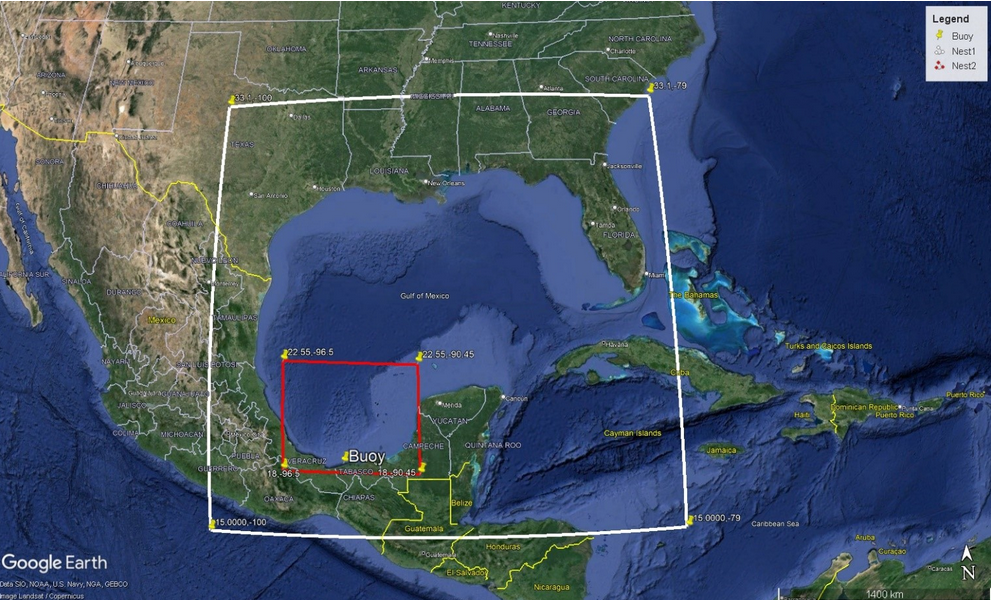
\includegraphics[width = .8\textwidth]{figures/modelDomain}
\caption{Model domains shown on map.}
\label{fig:domain}
\end{figure}
\comment{}{All figures: Figures usually precede first reference in the text.}

Forecasts are produced at 12Z each day, and run up to seven days ahead. Fugro have provided us with pre-computed forecast data for seven of these daily runs, with start dates spanning from 06/03/2022 to 12/03/2022. A schematic of this process is shown in figure \ref{fig:fugrosetup}. As stated in section \ref{sec:kalmanfilters}, we are unable to run the forecast model in this project, so each 7-day forecast window is treated separately with a single analysis step.

\begin{figure}[h]
\centering
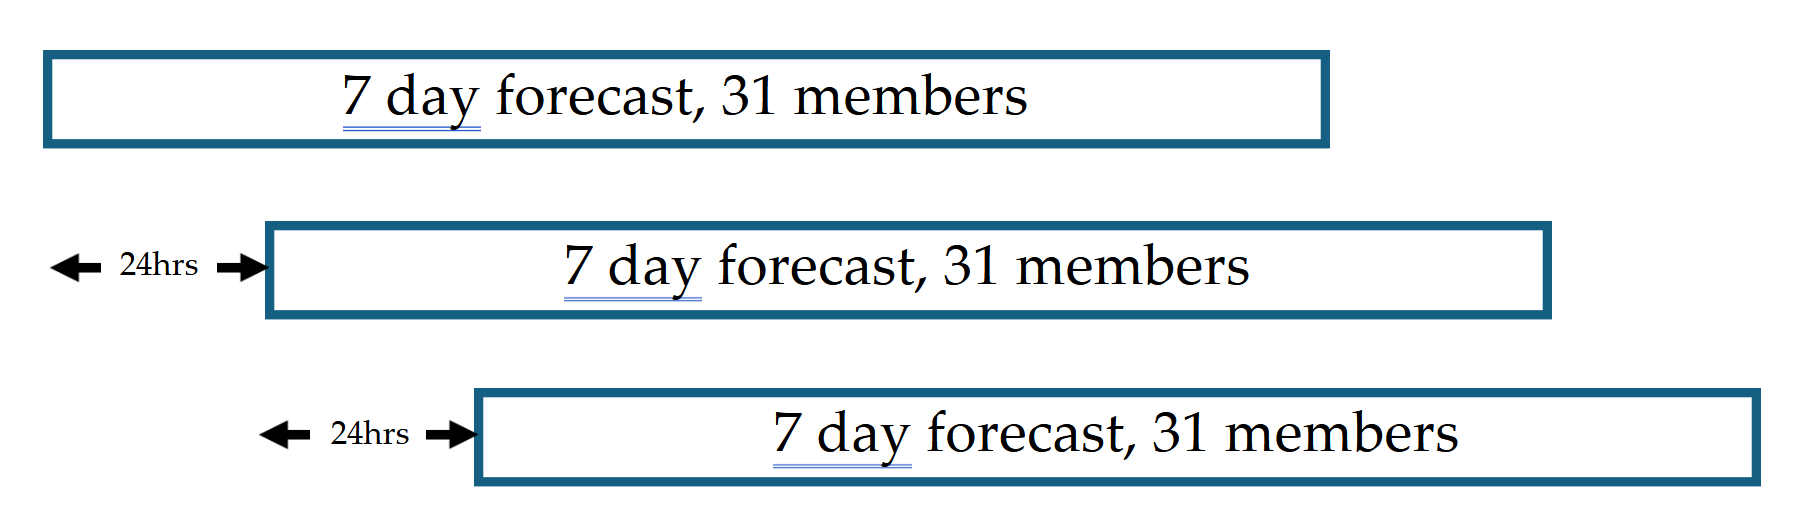
\includegraphics[width = .9\textwidth]{figures/fugrosetup}
\caption{Schematic of the forecasting setup used by Fugro. A new 7-day 31-member ensemble forecast is produced at 12Z each day.}
\label{fig:fugrosetup}
\end{figure}

%----------------------------------------------------------------------------------------
%	SECTION 2
%----------------------------------------------------------------------------------------

\section{Background State}
\label{sec:background}

The background state refers to the state of the system before DA, which in our case is given by the pre-computed forecast data from Fugro. In this section we present a general overview of the background state in the domain, across the period from 06/03/2022 to 19/03/2022. We identify the broad features of the waves in this window, and also discuss the effect of a cold front that passed through the region on 12/03/2022. This cold front is particularly important to consider as these events are a very common cause of high waves in the region, and in our examination of the results of this study we are particularly interested in forecasts of the waves associated with the cold front.

Figure \ref{fig:hdirtimemean} shows the significant wave height and direction averaged over the first six days and last six days of the forecast period. $H_s$ is mostly between 1m and 2m in the central gulf, with lower wave heights of < 1m in sheltered coastal areas such as the western side of Florida and the Yucatan peninsula. This is normal for the region according to \citet{Appendini2014}, in which a 30-year wave hindcast was constructed for the GoM using the MIKE 21 SW wave model \citep{Sorensen2004} forced by winds from the North American regional reanalysis \citep{Mesinger2006}. In that study, it was found that mean $H_s$ in the GoM is generally in the range 1m - 1.5m, with lower values < 1m in the shallow coastal waters.

The central part of the domain has largely east-southeasterly waves over both periods, which diverge after they pass between Yucatan and Cuba. The two periods are separated by the passage of strong cold front (figure \ref{fig:wavesandchart}) and there is a slight shift to more easterly waves after the front has passed. This change is likely related to the wind backing associated with the front. The southern part of the Gulf of Mexico has slightly higher waves, around 1 - 1.5m, in the six day period after the passage of the front.

\begin{figure}
\centering
\begin{subfigure}{.45\textwidth}
\centering
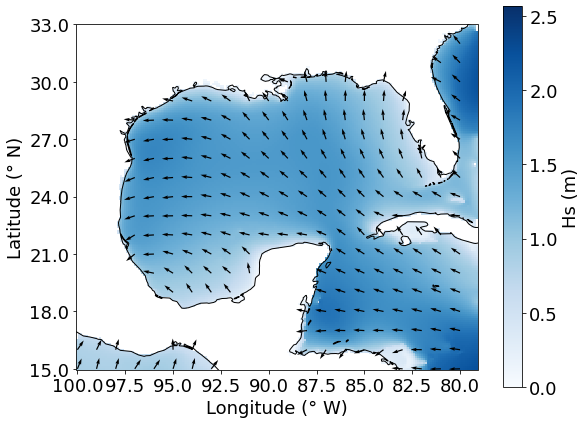
\includegraphics[width = \textwidth]{figures/hdir6-12}
\end{subfigure}
\begin{subfigure}{.45\textwidth}
\centering
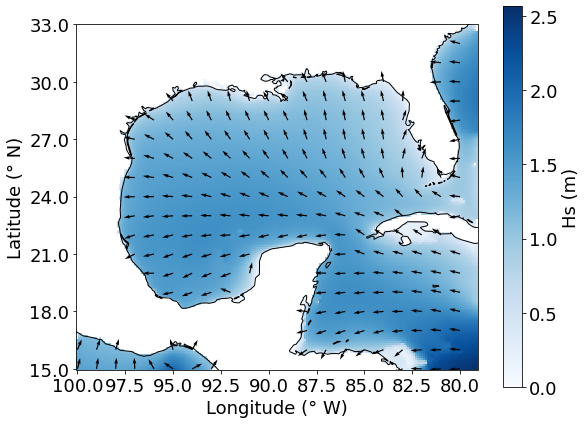
\includegraphics[width = \textwidth]{figures/hdir13-19}
\end{subfigure}
\caption{Left: $H_s$ (colours) and wave direction (arrows) averaged between 12Z 06/03/2022 and 12Z 12/03/2022. Right: The same averaged between 12Z 13/03/2022 and 12Z 19/03/2022}
\label{fig:hdirtimemean}
\end{figure}

There is a large peak in significant wave height on the 12/03/2022, related to a cold front passing through the region. A map of $H_s$ in the GoM at 18:00 on 06/03/2022 is shown in figure \ref{fig:wavesandchart}, along with a surface chart from the same time. The cold front is visible on the chart, and high waves are present in a large region behind the front. This is again in line with \citet{Appendini2014}, in which cold fronts are identified as a common driver of high waves between October and April, with the most intense peaks occuring between December and March.

The height of the waves during this event is up to 6m. This is not unusual according to \citet{Panchang2013}, in which wave height extremes in the GoM are analysed. The authors discuss what they call the SWH100, being the maximum estimated significant wave height in a 100 year period. They estimate SWH100 using multiple methods and in each case find that SWH100 is >10m in much of the central Gulf. The proximity of large $H_s$ values to the Southern coast of the GoM is slightly more unusual to see, as \citet{Panchang2013} finds SWH100 to be $\sim$ 7m much of the Southern GoM.The $H_s$ values seen here are still within this limit, but not by as much, indicating that the magnitude of wave heights forecast in this region may be unusual from a climatological standpoint.

\begin{figure}
\centering
\begin{subfigure}{.45\textwidth}
\centering
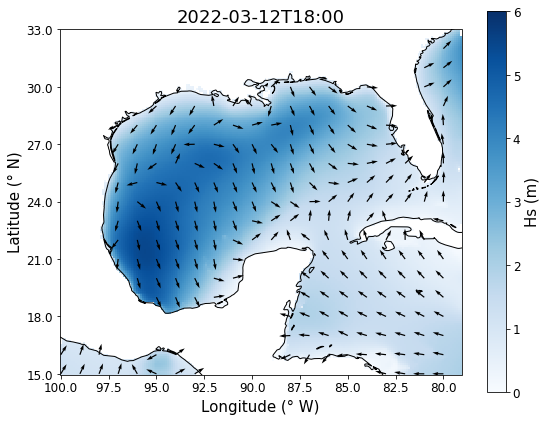
\includegraphics[width = \textwidth]{figures/0312waves}
\end{subfigure}
\hfill
\begin{subfigure}{.45\textwidth}
\centering
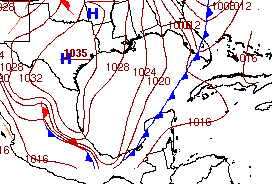
\includegraphics[width = \textwidth]{figures/0312chart}
\end{subfigure}
\caption{Left: \comment{$H_s$}{I would replace Hs in captions with significant wave height} (colours) and direction (arrows) in the GoM at 18Z on 12/03/2022. Right: Surface analysis chart valid for 18Z on 12/03/2022, taken from NOAA WPC surface analysis archive}
\label{fig:wavesandchart}
\end{figure}

Figure \ref{fig:t01maps} shows $T_{m01}$ at 18Z 12/03/2022 and averaged over the preceding 48 hours. The high waves associated with the cold front at 18Z have a period of $\sim$ 8s, which is higher than the period in the rest of the GoM at that time and also higher than the waves across the entire GoM in the 48 hours prior. This is also high compared to climatology, since \citet{Appendini2014} finds the average period in the region to be $\sim$ 6m.

\begin{figure}
\centering

\includegraphics[width = \textwidth]{figures/backgroundt01map}
\caption{Left: $T_{m01}$ at 18Z on 12/03/2022. Right: $T_{m01}$ averaged over the period from 12Z 10/03/2022 to 12Z 12/03/2022}
\label{fig:t01maps}
\end{figure}

In summary, we have seen that the wave heights during the forecast window were normal for the region, with the exception of those induced by a cold front on 12/03/2022. The waves associated with this cold front had longer period than most waves in the region, and the wave heights seen in the Southern GoM were somewhat climatologically unusual. We view this cold front event as particularly worthy of analysis, since it is this kind of event that poses a danger to offshore operations. This is especially true looking forward since \cite{Appendini2014} determined that extreme wave heights in the region are becoming higher over time.

%----------------------------------------------------------------------------------------
%	SECTION 3
%----------------------------------------------------------------------------------------

\section{Buoy Observations}
\label{sec:observations}

This section gives an overview of the buoy observations used in this study. The observations are a crucial part of DA as they give information about the true state of the system which can be used to improve forecasts. The equipments and methods used to generate the observations are discussed, as well as patterns and properties of the observational data.

Our observations come from an acoustic Doppler current profiler (ADCP) buoy (cite dissertation), which estimates the spectrum by measuring the wave induced velocity and surface height variations. According to \citet{Vallis2017}, the velocity and surface height anomaly induced by a simple wave with wave vector $\mathbf{k} = \left(k_x,k_y\right)$, frequency $\sigma$ and amplitude $a$ is

\begin{align*}
	u &= a \frac {k_x} {\sigma} g \exp{i(\mathbf{k}\cdot\mathbf{x} - \sigma t)} \cosh k(z + D) \\
	v &= a \frac {k_y} {\sigma} g \exp{i(\mathbf{k}\cdot\mathbf{x} - \sigma t)} \cosh k(z + D) \\
	w &= -i a \frac k \sigma g \exp{i(\mathbf{k}\cdot\mathbf{x} - \sigma t)} \sinh k(z + D) \\
	\eta &= a \exp{i(\mathbf{k}\cdot\mathbf{x} - \sigma t)}
\end{align*}

where only the real part of each expression should be taken. Note that the horizontal velocity $(u,v)$ is always in the same direction as the wave vector $\mathbf{k}$. From the ADCP measurements, a timeseries of surface height variance $\overline{\eta^2}$ can be calculated. This is related to the wave spectrum by equation \ref{eqn:waveenergy}, so a Fourier transform of $\overline{\eta^2}$ gives the direction-integrated spectrum $S(\sigma) = \int F(\sigma,\theta) \intd\theta$. Other variables are then deduced from this spectrum, including $H_s$, $T_{m01}$ and $T_{m02}$ as described above.

We have observations available over a roughly 6 month period spanning from October 2021 to April 2022, which includes the period for which forecasts are available. A timeseries of the observed significant wave height from the forecast period is included in figure \ref{fig:obshsseries}. The peak in wave height late on the 12th of March is clearly visible on the plot.

\begin{figure}[h]
\centering
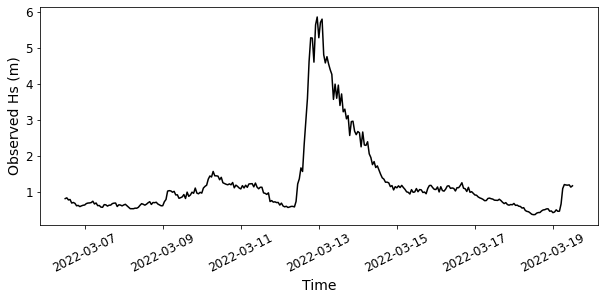
\includegraphics[width = .8\textwidth]{figures/obshsseries}
\caption{Observed timeseries of significant wave height from ADCP buoy}
\label{fig:obshsseries}
\end{figure}

Figure \ref{fig:buoyseries} shows a timeseries of observed $H_s$ and $T_{m01}$ from a longer period. We see that outside of specific peaks, $H_s$ is generally < 1m. This is consistent with the model background state which showed $H_s$ in the buoy region to be < 1m for much of the forecast period. The peaks generally consist of a sharp increase in $H_s$ followed by a more gradual decrease down to the baseline level. This is consistent with the slightly higher waves seen in the model background state in the buoy region after the passage of the front. As seen in the background state, the peaks in $H_s$ are associated with peaks in $T_{m01}$. This points to a positive correlation between $H_s$ and $T_{m01}$ which is dicussed further in section \ref{sec:bgerrors}.

\begin{figure}[h]
\centering
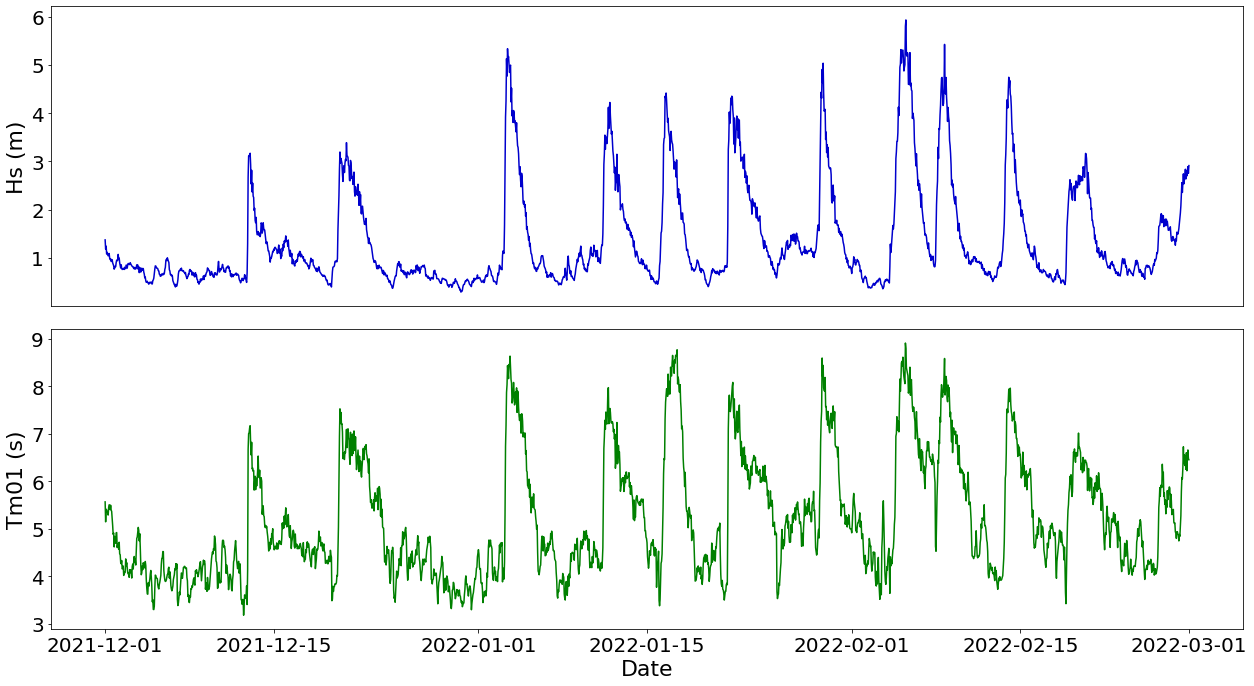
\includegraphics[width = \textwidth]{figures/buoyseries}
\caption{Timeseries of observed $H_s$ (top) and $T_{m01}$ (bottom) over a three-month period from 01/12/2021 to 01/03/2022}
\label{fig:buoyseries}
\end{figure}

Figure \ref{fig:obsdensityplot} shows a \comment{density plot}{Explain in more detail what you mean by density here. Is it a probability density, i.e. will it integrate to one or is it a relative frequency?} of observed $H_s$ and wave direction at the buoy location. There is a clear peak in frequency corresponding to waves of height $\sim$ 0.5m coming from \comment{a northeasterly direction}{In the previous section you called this southwesterly wave. This might be confusing. I would suggest changing to "waves from the northeast". Check this throughout}. Some higher waves (up to $\sim$ 5m) are present coming from a north-northwesterly direction. This lines up with the direction of waves produced by the cold front on 12/03/2022, suggesting that the waves produced by this kind of event consistently reach the buoy from a north-northwesterly direction. Since the buoy is near the coast in the southern part of the gulf, it is sheltered from the south so there are virtually no waves coming from this direction.

\begin{figure}[h]
\centering
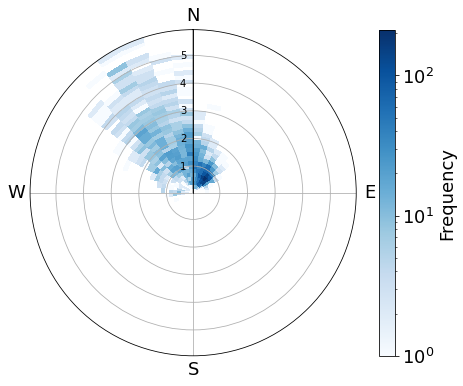
\includegraphics[width = .6\textwidth]{figures/obsdensityplot}
\caption{Density plot of $H_s$ (radial axis) and wave direction at the buoy location.}
\label{fig:obsdensityplot}
\end{figure}

%----------------------------------------------------------------------------------------
%	SECTION 4
%----------------------------------------------------------------------------------------

\section{Twin Experiment}
\label{sec:twinexp}

A twin experiment, also known as an observing system simulation experiment (OSSE), is a popular methodology often used for evaluating the impact of new observing systems when observational data is not yet available \citep{Zeng2020}. Even though we do have observations available, we use the OSSE methodology because (domain wide truth is not avilable in a realistic setup.)

In an OSSE, data from a model run (often called the `nature run', here called the `truth') is assimilated in place of real observational data. \comment{Here we select one of the 31 ensemble members}{Is it the same ensemble member in each window. Does the member change drastically between windows?} to represent the truth, and DA is applied to the remaining 30 ensemble members.

The observations are generated by sampling values from the truth at predefined observation locations and times. Here we sample hourly values from the nearest gridpoint to the buoy to match the real observations that are available. To represent observation error, some random noise is added to the sampled values. This noise is drawn from a normal distribution with standard deviation equal to the error standard deviation derived in section \ref{sec:obserrors}

(add into first paragraph) An advantage of this method in this context is that the `truth' is available away from the location of observations. This means that forecast error can be calculated over the whole model domain, which allows the effectiveness of DA to improve forecasts away from observation locations to be evaluated.

A downside of using the twin experiment method in this project is its inability to correct biases in the model. Figure \ref{fig:hsominusb} shows a possible bias in the forecasted values of $H_s$, which would be desirable to try to correct with DA. \comment{Since the data that we assimilate in this project is also from model output, it will be subject to all the same biases as the forecast data so it is not possible for the DA to correct these biases.}{Theoretically, you could add a bias to the the truth and see whether the DA can correct it. For simplicity, we haven't looked into a bias correcting scheme. You might want to mention that bias correcting DA schemes exist (the MetOffice has one) and then add some references to papers using them. }

%----------------------------------------------------------------------------------------
%	SECTION 5
%----------------------------------------------------------------------------------------

\section{Data Assimilation Setup}
\label{sec:DAsetup}

To perform the data assimilation , we use pyPDAF \citep{Chen2024}, which is a python interface for the 
Fortran-based Parallel Data Assimilation Framework (PDAF). We will use the update step from the ETKF method which comes builtin with PDAF. As previously stated, we do not have access to WW3, which makes a conventional  \replace{forecast}{prediction} step impossible. To get around this, at each analysis step we correct an entire 7-day forecast window, and in place of the forecast step we load data from the next forecast window. A schematic of the process is included in figure \ref{fig:ETKFschematic}. \add{So, in our setup, each 7-day window constituents a stand-alone DA problem with its own truth. In particular, improvements in one window are not propagated to the next.} 

\comment{This approach requires augmenting the state vector to include components from each leadtime within the forecast window.}{Preceding this sentence add information that you're using an ensemble smoother. That this implies that you are assimilating observations from different times and that because of this you have work with 4D vectors. I wouldn't call it augmenting, because you're concatenating. Next to this, I still think it is a good idea to write out the state vector here} %$()\x^{(n)})^\T=[(\x^{(n)})^\T(t=0),\dots,(\x^{(n)})^\T(7days)]$.}
 In this way, leadtime is treated the same as the two spatial coordinates by the DA system. At each analysis step, we will assimilate observations from the first three days of the forecast window. This allows us to investigate errors at times after the assimilation window and assess the capability of DA to improve the forecast at future time when observations are unavailable.

\comment{}{It would be better to depict every window as a bar divided into a part with assimilated observations and forecast with the bars staggered to reflect that the windows are one day apart and also add truth and observations taken from truth to the figure.}
\begin{figure}[h]
\centering
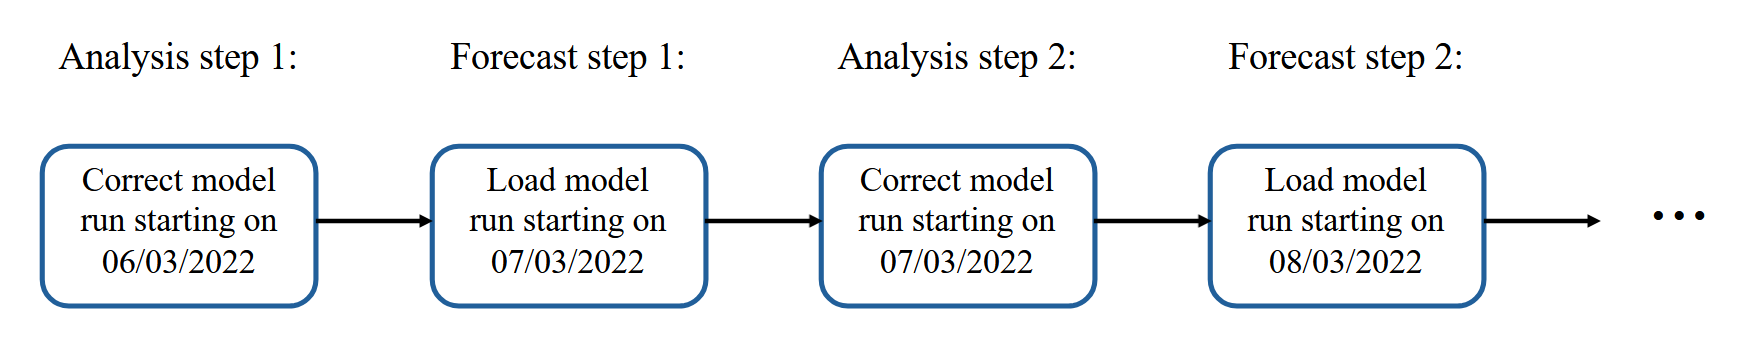
\includegraphics[width = \textwidth]{figures/ETKFschematic}
\caption{Schematic of the forecast and analysis steps from the \comment{ETKF scheme}{Don't call it ETKF scheme}.}
\label{fig:ETKFschematic}
\end{figure}

\section{Chapter Summary}

In this chapter, we have seen............